\chapter{Материалы и методы} \label{chapt1}

\section{Материалы} \label{sect1_1}



\section{Методы} \label{sect1_2}

\subsection{Выделение ДНК} \label{subsect1_2_1}

Образцы поступили будучи «законсервированными» в спирт, поэтому первым этапом было центрифугирование образцов при 5000g при температуре $4^{\circ}$ в течение 15 минут. Затем супернатант (SN) переносили в новую пробирку. Далее произодилось выделение ДНК из образованного осадка. К осадку добавляли 800 мкл лизирующего буфера (SDS) и 300 мг кремне-циркониевых бусин диаметром 0,1 мм и 100 мг – диаметром 0,5 мм. Затем гомогенизировали на Beadbeaten, после чего инкубировали при $70^{\circ}$ в течение 15 минут. Далее снова центрифугировали на максимальных оборотах 15 минут и переносили образовавшийся SN в новую пробирку. Добавляли к SN равный объем изопропанола, перемешивая переворачиванием. После инкубировали не менее часа при $-20^{\circ}$. Далее центрифугировали на максимальных оборотах 30 минут при температуре $4^{\circ}$ . Полученный осадок давжды промывали 70\% спиртом и высушивали при комнатной температуре 15 минут. После растворяли в 100 мкл ТЕ-буфера. 

Так же возможно выделение ДНК из спирта, в котором хранились образцы. После первого центрифугирования (5000g, 15 мин, $4^{\circ}$) к SN добавляется два объема спирта и один объем 3М ацетата Na. Далее образцы инкубируются не менее часа при $-20^{\circ}$, после чего снова центрифугируются на максимальных оборотах в течение 30 минут при $4^{\circ}$. Далее осадок дважды промывается в 70\% спирте и высушивается при комнатной температуре 15 минут. Затем осадок растворятся в ТЕ-буфере. 

После выделения ДНК производилось приготовление библиотеки к секвенированию.

\subsection{Секвенирование вариабельных участков V3-V4, V5-V6 гена 16S рРНК}  \label{subsect1_2_2}

Приготовление ампликонных библиотек на вариабельные участки V3-V4, V5-V6 (?) проводилось  в соответствии с протоколом, рекомендуемым компанией Illumina , \textit{16S Metagenomic Sequencing Library Preparation }

Была проведена  двустадийная поимеразная цепная реакция (ПЦР) (см. рис. \ref{img:two_stage_pcr}). Для каждого образца составлялась смесь общим объемом 25 мкл, содержавшая 1 мкл ДНК, 1мкл каждого из двух праймеров (10 пмоль), 2,5 мкл 10х буфера для ПЦР, 2,5 мкл dNTP, 0,5 мкл  Taq-полимеразы и 16,5 мкл воды. Далее проводили реакцю при следующих условиях:
\begin{enumerate}
	\item $95^{\circ}$ , 3 мин – денатурация;
	\item 25 циклов:
	\begin{itemize}
		\item $95^{\circ}$, 30 с – денатурация
		\item $55^{\circ}$, 30 с – отжиг праймеров на матрице
		\item $72^{\circ}$, 30 с – элонгация	
	\end{itemize}
	\item $72^{\circ}$, 5 мин – ?
	\item  $4^{\circ}$ ,  $\infty$ 
\end{enumerate}

\begin{figure}[h]
  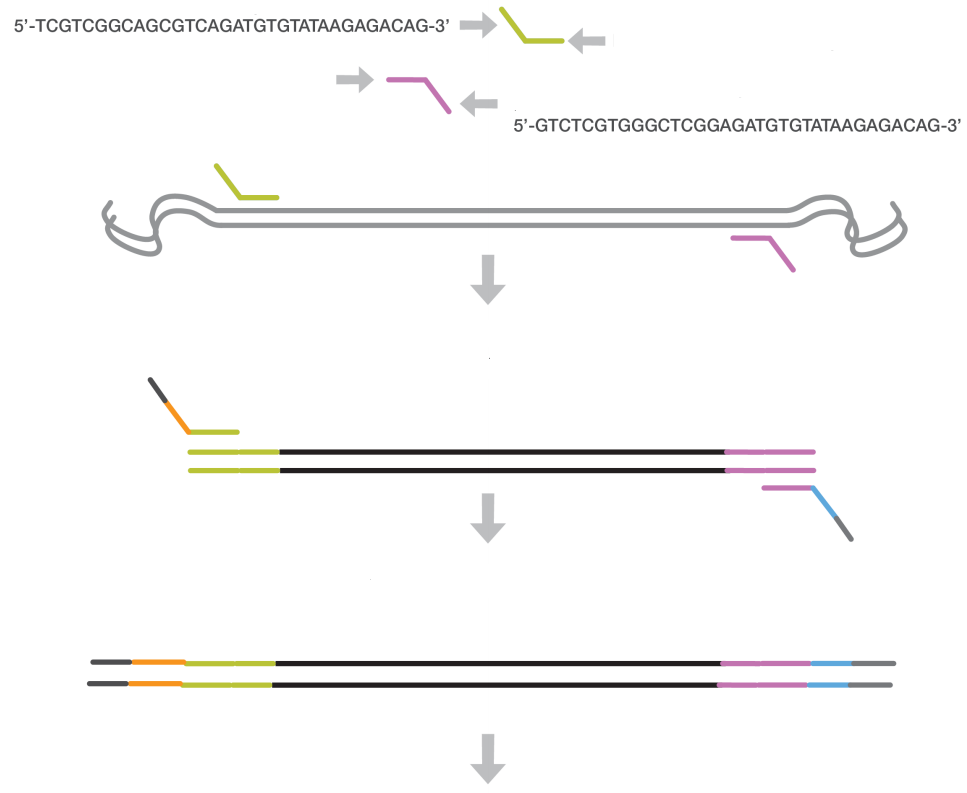
\includegraphics[width=8cm]{two_stage_pcr}
  \centering
  \caption{Двустадийная ПЦР}
  \label{img:two_stage_pcr}  
\end{figure}

После следовала чистка ампликонов от свободных праймеров и димеров с использованием AMPure XP beads. Далее для проверки того, что ПЦР прошла хорошо ставили электрофорез в агарозном геле. 

После того, как были выбраны накоплены необходимые вариабельные участки, шла вторая стадия ПЦР, на которой к образцам пришивались индексированные праймеры.  Для каждого образца составлялась смесь общим объемом 50 мкл, которая содержала 5 мкл матрицы, 5 мкл буфера для ПЦР, 5 мкл dNTP, по 1 мкл каждого из двух индексированных праймеров, 0,5 мкл полимеразы и 32,5 мкл воды. Далее проводили реакцю при следующих условиях:
\begin{enumerate}
	\item $95^{\circ}$ , 3 мин – денатурация;
	\item 8 циклов:
	\begin{itemize}
		\item $95^{\circ}$, 30 с – денатурация
		\item $55^{\circ}$, 30 с – отжиг праймеров на матрице
		\item $72^{\circ}$, 30 с – элонгация
	\end{itemize}
	\item $72^{\circ}$, 5 мин – ?
	\item $4^{\circ}$ ,  $\infty$
\end{enumerate}

После полученные библиотеки снова проходили этап чистки с AMPure XP beads. 
Далее образцы анализировались с использованием Bioanalyzer DNA 1000 chip для проверки размера полученной библиотеки (~630п.о.). 

Далее образцы смешивались в эквимолярном соотношении: рассчитывается концентрация ДНК в нМ, определенная Agilent Technologies 2100 Bioanalyzer.

\begin{equation}
\dfrac{\text{концентрация в нг/мкл}}{\text{660 г/моль \* средний размер библиотеки}}\*10^6=\text{концентрация в нМ}
\end{equation}

\vspace{\baselineskip}

После следовала стадия секвенирования. 

\subsection{Секвенирование вариабельных участков V2-4-8/ V3-V6,V7-9 гена 16S рРНК}  \label{subsect1_2_3}

Приготовление библиотеки происходило в соответсвии с протоколом \textit{Ion} $16S^{TM}$ \textit{ Metagenomics Kit} (см. рис. \ref{img:workflow}). Было использовано два набора праймеров для вариабельных участков V2-4-8/ V3-V6,V7-9. 

\begin{figure}[h]
  \includegraphics[width=8cm]{workflow}
  \centering
  \caption{Алгоритм работы по протоколу Ion $16S^{TM}$ Metagenomics Kit }
  \label{img:workflow}  
\end{figure}

Для получения необходимых ампликонов была проведена ПЦР. Для кажого образца замешивалась смесь, общим объемом 30 мкл, которая содержала 15 мкл 2X Environmental Master Mix, 3 мкл 16S Primer Set $(10X)^{[1]}$, 2-12 мкл образца, объем воды, необходимый до 30 мкл.  Далее проводили реакцю при следующих условиях:

\begin{enumerate}
	\item $95^{\circ}$ , 10 мин – денатурация;
	\item 18-25 циклов:
	\begin{itemize}
		\item $95^{\circ}$, 30 с – денатурация
		\item $58^{\circ}$, 30 с – отжиг праймеров на матрице
		\item $72^{\circ}$, 20 с – элонгация
	\end{itemize}
	\item $72^{\circ}$, 7 мин – ?
	\item $4^{\circ}$ ,  $\infty$
\end{enumerate}

После следовала чистка ампликонов от свободных праймеров и димеров с использованием AMPure XP beads. Затем выравнивали концы ампликонов, инкубируя их при комнатной температуре в течение 20 минут с использованием 5X End Repair Buffer и End Repair Enzyme . Затем снова была чистка ампликонов от свободных праймеров и димеров с использованием AMPure XP beads. Затем были лигированы адаптеры и проведена никтрансляция. Для этого была проведена ПЦР. Для кажого образца замешивалась смесь, общим объемом 100 мкл, которая содержала 25 мкл матрицы, 10 мкл 10X Ligase Buffer, 2 мкл Ion P1 Adapter, 2 мкл Ion Xpress™ Barcode X[1] , 2 мкл dNTP Mix, 49 мкл Nuclease-free Water, 2 мкл DNA Ligase, 8 мкл Nick Repair Polymerase.   Далее проводили реакцю при следующих условиях:

\begin{enumerate}
	\item $25^{\circ}$ , 15 мин;
	\item $72^{\circ}$, 5 мин;
	\item $4^{\circ}$ ,  $\infty$.
\end{enumerate}

После следовала чистка ампликонов от свободных праймеров и димеров с использованием AMPure XP beads. Затем измеряли концентрацию, используя Qubit, проверяли качество библиотеки на Bioanalyzer DNA HS chip. Разводили библиотеки до концентрации 100 пмоль, смешивали в эквимолярном соотношении (аналогично протоколу Illumina). Далее следовала эмульсионная ПЦР, чтобы посадить фрагментную библиотеку на специальные шарики, которые впоследствии будут нанесены на чип для секвенирования. Так как данный процесс имеет погрешность, то есть не все шарики оказываются связанными с бибилотекой, то была проведена процедура обогощения, в процессе которой мы избавились от пустых шариков. Затем следовало нанесение уже обогощенной баблиотеки на чип, и далее было проведено секвенирование.




\subsection{Shotgun-секвенирование}  \label{subsect1_2_4}
Приготовление библиотеки происходило в соответсвии с протоколом $IonXpress^{TM}$ \textit{Plus gDNA Fragment Library Preparation}.

Выделенную ДНК необходимо было поделить на фрагменты длинной 200 пар оснований. Данный этап происходил с использованием Covaris. После необходимо выровнять концы фрагментов, для этого была проведена инкубация при комнатной температуре с использование  \textit{5X End Repair Buffer} и  \textit{End Repair Enzyme}. Избавление от димеров и фрагментов малой длины (\~50 п.о.) происходило при чистке с использованием \textit{Agencourt AMPure XP Kit}. Следующим этапом было лигирование адаптеров и никтрансляция. Для этого ставилась ПЦР. Для каждого образца замешивалась смесь общим объемом 100 мкл, которую впоследствии делили на две пробирки одинакового объема для лучшего протекания реакции. Каждая пробирка содеражала 25 мкл ДНК, 10 мкл 10X Ligase Buffer, 2 мкл Ion P1 Adapter, 2 мкл Ion Xpress Barcode X, 2 мкл dNTP Mix, 49 мкл Nuclease-free Water, 2 мкл DNA Ligase, 8 мкл Nick Repair Polymerase. 

Далее проводили реакцю при следующих условиях для одного цикла:

\begin{enumerate}
	\item $25^{\circ}$ , 15 мин;
	\item $72^{\circ}$ , 5 мин;
	\item $4^{\circ}$ ,  $\infty$.
\end{enumerate}

Далее была чистка от димеров с использованием \textit{Agencourt AMPure XP Kit}.

Так как существует большая погрешность при фрагментации и не все фрагменты получаются одинаковой длины, то очищение от фрагментов большой длины (\~100 п.о.) происходит с использование агарозного E-Gel. Данный этап работы называется size-select. Затем снова проводилась амплификация, чтобы увеличить концентрацию фрагментов с лигированными адаптерами. Для каждого образца замешивалась смесь общим объемом 130 мкл, которую впоследствии делили на две пробирки одинакового объема для лучшего протекания реакции. Каждая пробирка содеражала 100 мкл Platinum PCR SuoerMix High Fidelity, 5 мкл Library Amplification Primer Mix, 25 мкл неамплифицированной библиотеки. 

Далее проводили реакцю при следующих условиях для одного цикла:

\begin{enumerate}
	\item $95^{\circ}$ , 5 мин 
	\item n циклов:
	\begin{itemize}
		\item $95^{\circ}$, 15 с – денатурация
		\item $58^{\circ}$, 15 с – отжиг праймеров на матрице
		\item $70^{\circ}$, 1 мин – элонгация
	\end{itemize}
	\item $4^{\circ}$ ,  $\infty$
\end{enumerate}

Далее снова чистили библиотеки, измеряли концентрацию, используя Qubit, проверяли качество библиотеки на Bioanalyzer DNA HS chip. Разводили библиотеки до концентрации 100 пмоль, смешивали в эквимолярном соотношении (аналогично протоколу Illumina). Далее следовала эмульсионная ПЦР, чтобы посадить фрагментную библиотеку на специальные шарики, которые впоследствии будут нанесены на чип для секвенирования. Так как данный процесс имеет погрешность, то есть не все шарики оказываются связанными с бибилотекой, то была проведена процедура обогощения, в процессе которой мы избавились от пустых шариков. Затем следовало нанесение уже обогощенной баблиотеки на чип, и далее было проведено секвенирование. 


\subsection{Анализ полученных данных}  \label{subsect1_2_5}

Данные, полученые с Illumina MiSeq, были обработаны програмным обеспечением, встроенным в прибор. Также была использована база данных по гену 16S рРНК GreenGenes. Для последующего анализа данные были визуализированны при помощи MEGAN5.

Полученные с IT PGM  риды по гену 16S рРНК были собраны ассемблером IDBA-UD. Контиги были собраны с использованием онлайн-сервера RDP. 


Shotgun-риды были собраны SPAdes Genome Assembler, проаннотированы с помощью баззы данных Prokka. Из Prokka были взяты EC-номера, и отправлены на анализ в KEGG, что дало возможность получить карты метаболических путей. Также была проведена визуализация при помощи MEGAN5.


\clearpage
